\documentclass{article}

\usepackage{graphicx}
\usepackage{tikz}
\usepackage{tikzsymbols}
\usetikzlibrary{calc,patterns,shapes.geometric}
\pagestyle{empty}
\usepackage[margin=0pt]{geometry}
\geometry{papersize={14in,12in}}

\def\centerarc[#1](#2)(#3:#4:#5){\draw[#1] ($(#2)+({#5*cos(#3)},{#5*sin(#3)})$) arc (#3:#4:#5);}

\begin{document}
	\begin{figure}
		\centering
		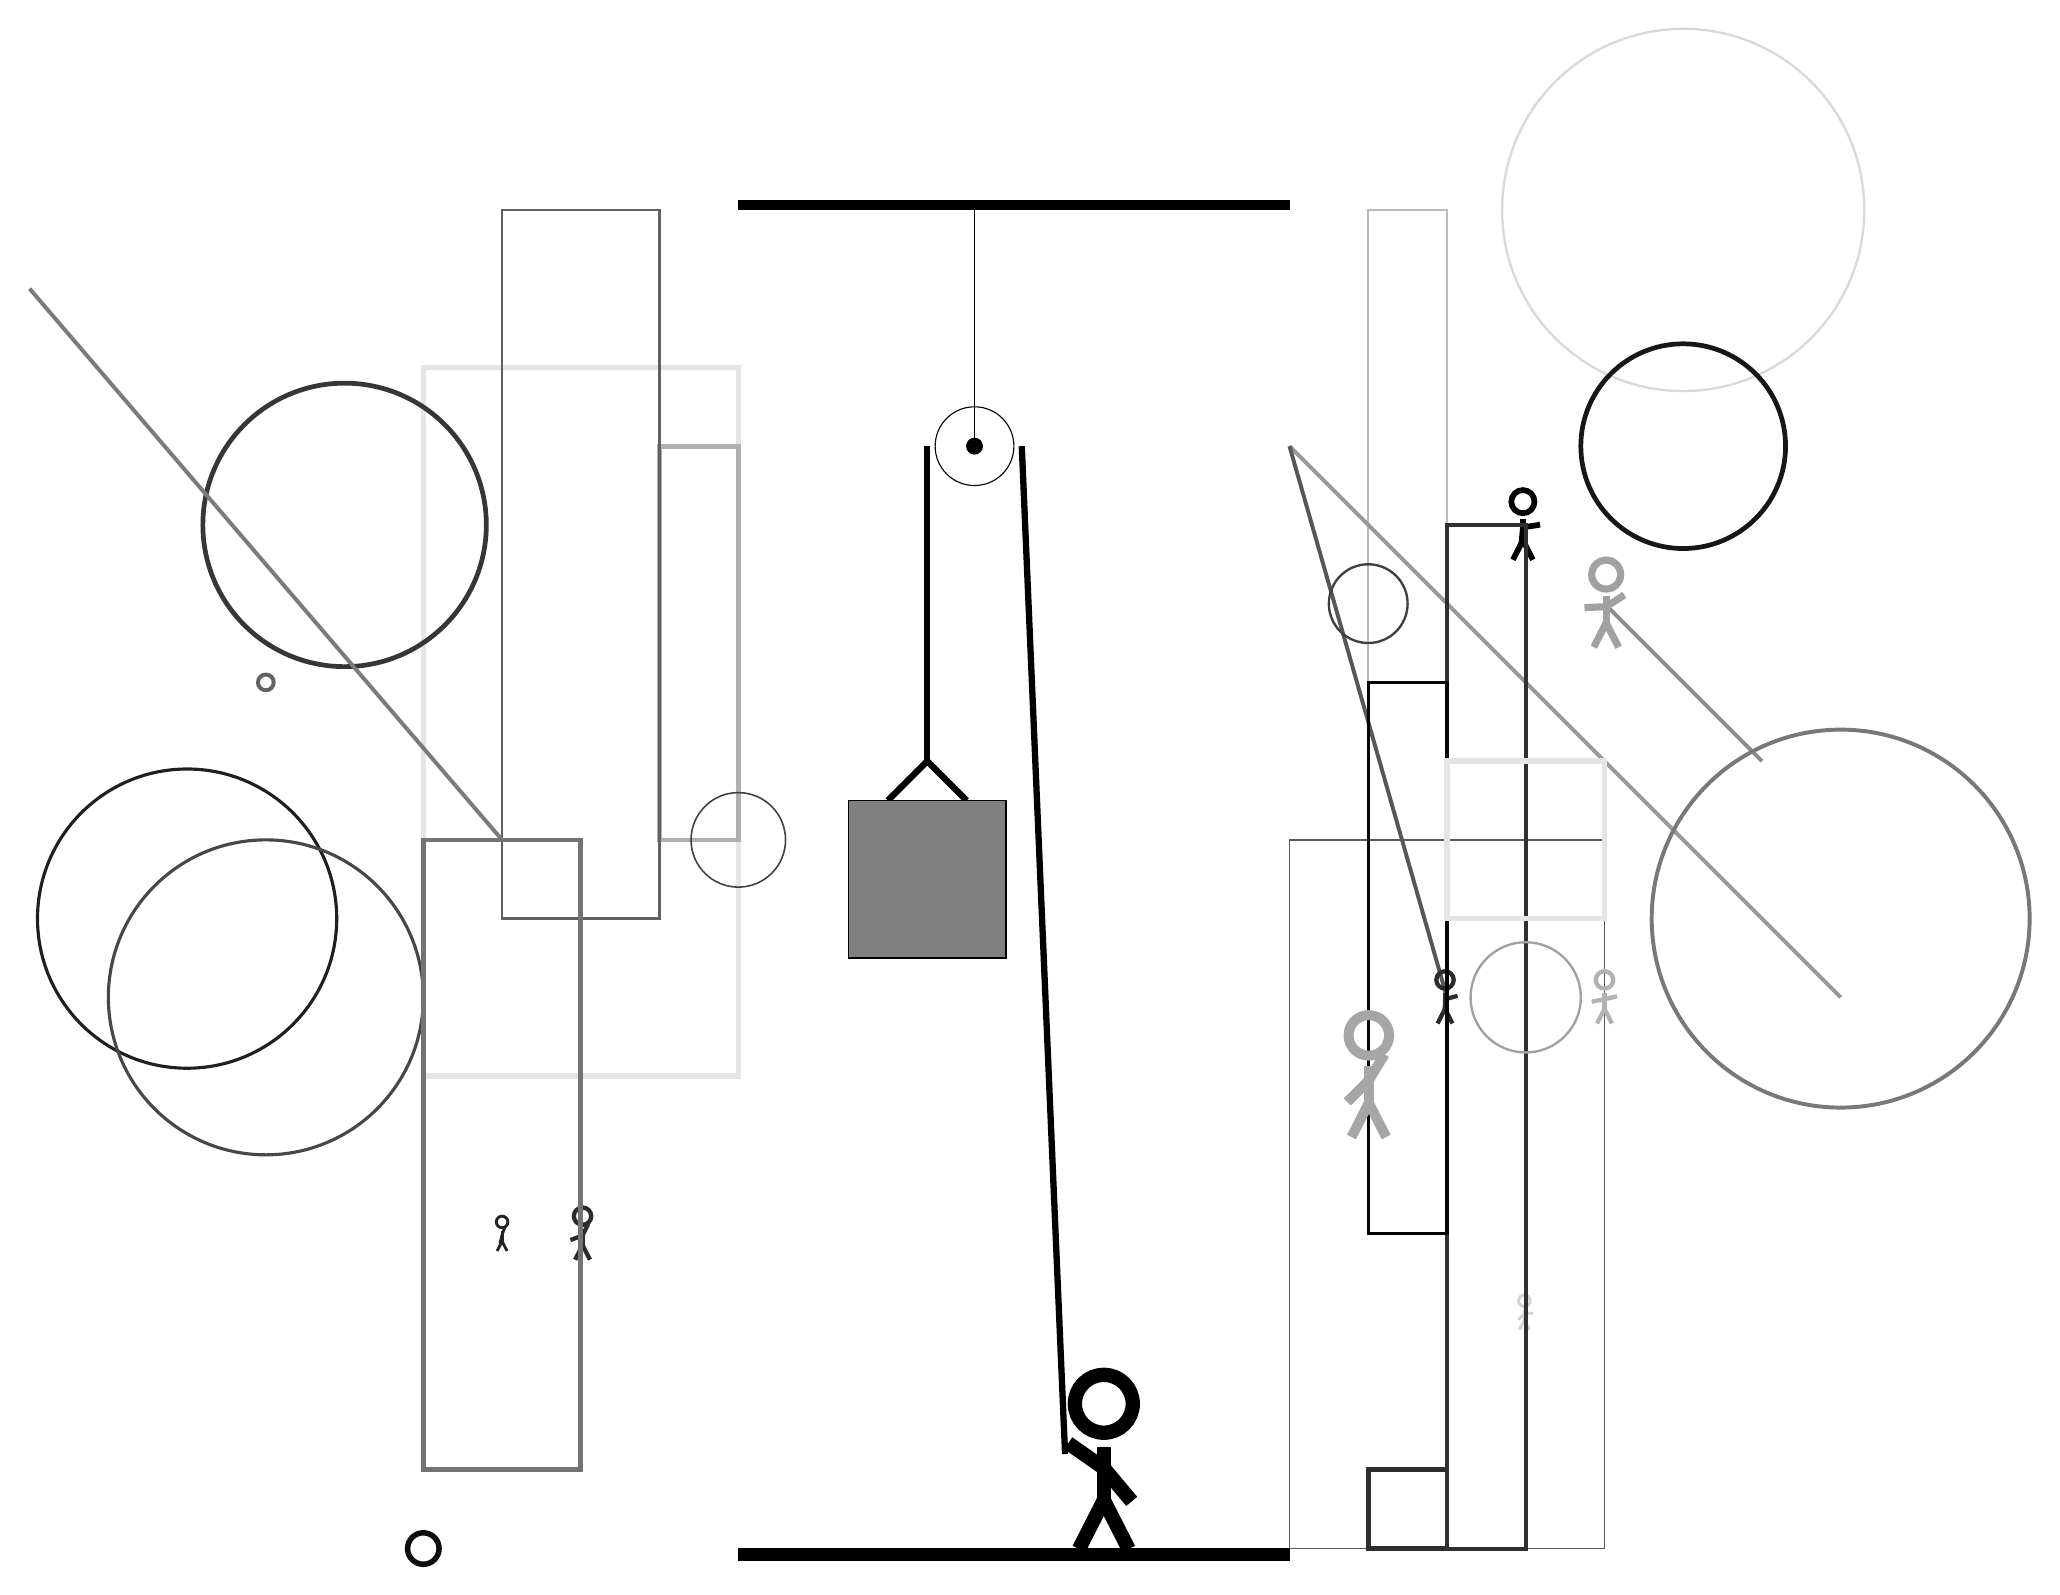
\begin{tikzpicture}
			%%%%% START %%%%%
			
			\draw[fill=black] (-2, 14) rectangle (5, 14.125);
			
			\draw (1, 11) circle (0.5);
			\draw[fill=black] (1, 11) circle (0.1);
			\draw (1, 14) -- (1, 11);
			
			\draw[line width=0.8mm] (-0.1, 6.5) -- (0.4, 7.0) -- (0.9, 6.5);
			\draw[fill=black!50] (-0.6, 6.5) rectangle (1.4, 4.5);
			
			\draw[line width=0.8mm] (0.4, 11) -- (0.4, 7.0);
			\centerarc[line width=0.8mm](1, 11)(0:180:0.6);
			\draw[line width=0.8mm](1.6, 11) -- (2.15, -1.8);
			
			\node at (2.6, -1.9) {\Strichmaxerl[10][-35][-50]};
			
			\draw[line width=0.7mm, color=black!10] (-2, 12) rectangle (-6, 3);
			
			\draw[line width=0.2mm, color=black!27] (6, 14) rectangle (7, 8);
			\draw[line width=0.2mm, color=black!65] (5, 6) rectangle (9, -3);
			\node[line width=0.5mm, color=black!99] at (8, 10) {\Strichmaxerl[4][85][9]};
			\draw [line width=0.3mm, color=black!15](10, 14) circle (2.3);
			\draw [line width=0.4mm, color=black!44](-7, 6) circle (0.0);
			
			\draw[line width=0.5mm, color=black!45](9, 9) -- (11, 7);
			
			\draw [line width=0.4mm, color=black!88](-9, 5) circle (1.9);
			\draw[line width=0.5mm, color=black!40](5, 11) -- (12, 4);
			
			\draw [line width=0.6mm, color=black!91](10, 11) circle (1.3);
			\node[line width=0.3mm, color=black!83] at (-4, 1) {\Strichmaxerl[3][21][64]};
			\draw [line width=0.4mm, color=black!72](-8, 4) circle (2.0);
			\draw[line width=0.6mm, color=black!31] (-2, 6) rectangle (-3, 11);
			\draw[line width=0.5mm, color=black!66](7, 4) -- (5, 11);
			\node[line width=0.4mm, color=black!83] at (7, 4) {\Strichmaxerl[3][89][15]};
			\node[line width=0.2mm, color=black!30] at (9, 4) {\Strichmaxerl[3][11][13]};
			\draw [line width=0.2mm, color=black!38](6, 12) circle (0.0);
			\draw [line width=0.6mm, color=black!79](-7, 10) circle (1.8);
			\draw [line width=0.7mm, color=black!95](-6, -3) circle (0.2);
			\draw [line width=0.5mm, color=black!61](-8, 8) circle (0.1);
			\node[line width=0.6mm, color=black!18] at (8, 0) {\Strichmaxerl[2][46][3]};
			\draw[line width=0.3mm, color=black!62] (-3, 14) rectangle (-5, 5);
			\draw [line width=0.5mm, color=black!53](12, 5) circle (2.4);
			\draw[line width=0.6mm, color=black!82] (7, -2) rectangle (6, -3);
			\draw[line width=0.5mm, color=black!81] (7, -3) rectangle (8, 10);
			\draw[line width=0.5mm, color=black!52](-5, 6) -- (-11, 13);
			
			\node[line width=0.2mm, color=black!86] at (-5, 1) {\Strichmaxerl[2][76][70]};
			\draw [line width=0.3mm, color=black!37](8, 4) circle (0.7);
			
			\draw[line width=0.4mm, color=black!98] (7, 8) rectangle (6, 1);
			
			\node[line width=0.5mm, color=black!35] at (6, 3) {\Strichmaxerl[7][45][59]};
			\draw[line width=0.4mm, color=black!98] (7, 8) rectangle (7, 4);
			
			\draw[line width=0.7mm, color=black!10] (7, 7) rectangle (9, 5);
			\node[line width=0.5mm, color=black!37] at (9, 9) {\Strichmaxerl[5][2][33]};
			\draw [line width=0.2mm, color=black!75](-2, 6) circle (0.6);
			\draw [line width=0.3mm, color=black!75](6, 9) circle (0.5);
			\draw[line width=0.6mm, color=black!55] (-4, 6) rectangle (-6, -2);
			
			\draw[fill=black] (-2, -3) rectangle (5, -3.15);
			
			%%%%% END %%%%%
		\end{tikzpicture}
	\end{figure}	
\end{document}